\documentclass[a4paper,12pt]{article}
\usepackage[table]{xcolor}
\usepackage{array,amsmath,amssymb,multicol,tikz}
\usepackage{hyperref,colonequals}
\usepackage[margin=2cm]{geometry}
\usepackage{fancyvrb}
\usetikzlibrary{calc,arrows.meta}
\usepackage{xcolor}

\tikzset{
arr/.style={line width=1pt,-{Straight Barb[width=6pt, length=3pt]}, shorten >=2pt}
}

\pagestyle{empty}

\newcommand\N{\mathbf{N}}
\newcommand\Q{\mathbf{Q}}
\newcommand\R{\mathbf{R}}
\newcommand\Z{\mathbf{Z}}

\newcommand\rem{\textup{rem}}

\setlength{\parindent}{0pt}

\begin{document}

\begin{center}
\parbox{3cm}{\flushleft\bf Discrete\linebreak Structures}
\hfill
\parbox{7cm}{\centering {\bf\Huge Samples, Part 2}}
\hfill
\parbox{3cm}{\flushright\bf Spring 2021 \linebreak May 25}
\end{center}

\hrule\vspace{2pt}\hrule

\hrule



\vspace{10pt}
{\bf Number Theory.}

\begin{enumerate}

% 1.(a)
\item {\small \em
Factorize a number into a product of prime powers.}\\
Express $1001000$ in the form $p_1^{k_1} p_2^{k_2} \cdots p_m^{k_m}$,
where all $p_i$ are different primes and $k_i$ are non-negative integers.


% 1.(b)
\item {\small \em
Divide numbers with remainders as in $n = qd + r$, express decimal digits.}\\
Assume that you have all $4$ arithmetic operations and also two
more operations: $\mathbf{div}$ (integer division) and $\mathbf{mod}$
(remainder).\\
For example $17\ \mathbf{div}\ 3 = 5$,
$(-17)\ \mathbf{div}\ 3 = -6$, $17\ \mathbf{mod}\ 3 = 2$,
$(-17)\ \mathbf{div}\ 3 = 1$.\\
{\em Note.} In Python $\mathbf{div}$ and $\mathbf{mod}$  are
written as {\tt 17//3} and {\tt 17\%3} respectively.

Let $n$ be a positive integer.
\begin{enumerate}
\item Express $n$ as $n = 7q + r$, where $r \in \{ 0,1,2,3,4,5,6 \}$,
but $q$ is any integer. Write formulas that express $q$ and $r$ for the given $n$.
\item Express the last binary digit of $n$ (it should be $0$ for even $n$
and $1$ for odd $n$).
\item
Write an expression $d_4(n)$ for the
4rd decimal digit (from the right). It should return $0$, if the number
$n$ has fewer than four decimal digits.\\
For example, $d_4(2345) = 2$
and $d_4(999) = 0$.
\item
Write an expression $h_3(n)$ for the 3rd hexadecimal digit (from the right).
And it should be $0$, if number does not have $3$ hexadecimal digits.\\
For example $h_3(\mathtt{37FF}_{16}) =7$; $h_3(\mathtt{7FFF}_{16}) = 15$,
and $h_3(\mathtt{FF}_{16}) = 0$.
\end{enumerate}

% 1.(c)
\item {\small \em
Find members of arithmetic progressions, also by modulo $m$.}\\
Let $(a_n)$ be an arithmetic progression defined by a recurrence:
$a_0 = 3$ and $a_{n+1} = a_n + 7$.
\begin{enumerate}
\item How many members of this progression are $3$-digit numbers
(i.e. numbers between $100$ and $999$)?
\item
What is the last digit of the member $a_{2021}$?
\end{enumerate}

% 1.(d)
\item {\small \em
Given two integers, find their GCD (also LCM) by Euclidean algorithm.}\\
\begin{enumerate}
\item
Write the Euclidean algorithm execution to find $\text{gcd}(1396,482)$.
\item
Express also $\text{lcm}(1396,482)$ \textendash{} the least common multiplier
of both numbers.
\item
The prime factorization for both numbers $7007$ and $9100$ are given:
\[ \left\{  \begin{array}{l}
7007 = 7^2 \cdot 11^1 \cdot 13^1,\\
9100 = 2^2 \cdot 5^2 \cdot 7^1 \cdot 13^1.\\
\end{array} \right. \]
Express the prime factorizations of the $\text{gcd}(7007,9100)$
and also  $\text{lcm}(7007,9100)$.
\end{enumerate}

% 1.(e)
\item {\small \em
Given integers, solve Bezout identity with Blankenship algorithm.}\\
Find a positive integer $d = \text{gcd}(106,16)$ and find some two integers $x,y$ that solve
the Bezout identity:
\[ 106x + 16y = d. \]



% 1.(f)
\item {\small \em
Given $m$ and $x$, compute
multiplicative inverse $\overline{x}$ modulo $m$; solve linear congruences.}\\
Assume that you need to solve several linear congruences $3x \equiv a$ modulo $37$
for various values of $a$.
\begin{equation}
\label{eq:linear-congruences}
\left\{ \begin{array}{l}
3x \equiv 5 \pmod{37} \\
3x \equiv 6 \pmod{37} \\
3x \equiv 7 \pmod{37} \\
3x \equiv 8 \pmod{37}
\end{array} \right.
\end{equation}
There is no division in modular arithmetic, but you can find inverse of $3$
modulo $37$ which is helpful to solve these congruences.
\begin{enumerate}
\item Find the multiplicative inverse of $3$ modulo $37$.
\item Solve any two congruences from (\ref{eq:linear-congruences}).
\end{enumerate}



% 1.(g)
\item {\small \em
Convert periodic decimal numbers to rational fractions.}\\
\begin{enumerate}
\item
Convert the periodic fraction $0.2021(235) = 0.2021235235\ldots$ into a rational
fraction $m/n$ where $m,n \in \Z$.
\item
Express the number $0.0000(235) = 0.0000235235\ldots$ as the sum
of infinite geometric series.
\end{enumerate}


% 1.(h)
\item {\small \em
Given a decimal integer, convert it to binary, hexadecimal (and vice versa).}\\
Convert $1000_{10}$ into binary and hexadecimal notation.
\end{enumerate}





\vspace{10pt}
{\bf Graphs.}

\begin{enumerate}
%2.(a)
\item {\small \em  Count the number of graphs with a given property or parameter.}\\
Count the number of graphs having exactly $4$ vertices and
exactly $3$ edges. (All graph vertices are considered unique;
graphs that differ by isomorphism are considered different graphs.)

%2.(b)
\item {\small \em  Justify whether or not a graph has a particular subgraph, cycle or path; whether or not some configuration is possible.}\\
Consider the full bipartite graph $K_{3,3}$ (two sets of $3$ vertices; all $9$ edges
that connect vertices between different sets belong to this graph).
\begin{enumerate}
\item Does it contain $C_4$ as a subgraph (a cycle with $4$ vertices)?
\item Does it contain $C_5$ as a subgraph (a cycle with $5$ vertices)?
\end{enumerate}

%2.(c)
\item {\small \em  Convert between graph representations.
Check if a graph is bipartite, complete, or connected. }\\
A graph $G(V,E)$ has $5$ vertices labeled with numbers: $V=\{ 0,1,2,3,4 \}$.
It has the following adjacency list representation:

\begin{figure}[!htb]
\center{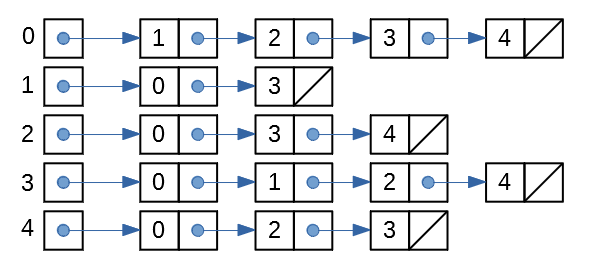
\includegraphics[width=2.5in]{figs/part2-graph-adjacency.png}}
\caption{\label{fig:part2-graph-adjacency} Adjacency lists for a graph.}
\end{figure}

\begin{enumerate}
\item Create the diagraph for this graph showing all the vertices and edges.
\item Create the matrix representation for this graph.
\end{enumerate}


%2.(d)
\item {\small \em  Given a tree, check the condition for a Euler circuit (or path) and find it.}\\
Figure~\ref{fig:part2-eulerian-graph} shows an undirected graph.
\begin{figure}[!htb]
\center{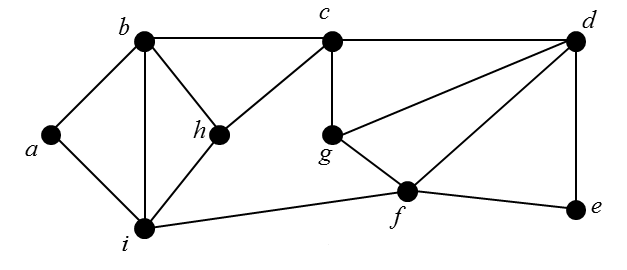
\includegraphics[width=2.5in]{figs/part2-eulerian-graph.png}}
\caption{\label{fig:part2-eulerian-graph} Graph to find Euler circuits or paths.}
\end{figure}
\begin{enumerate}
\item Does the graph have a Eulerian circuit? (Show the circuit or prove that it does
not exist.)
\item Does the graph have a Eulerian path? (Show the path or prove that it does
not exist.)
\end{enumerate}





%2.(e)
\item {\small \em  Given two graphs prove or disprove they are isomorphic.}\\
For the graph pairs shown in Figures~\ref{fig:part2-isomorphic-graphs1} and
\ref{fig:part2-isomorphic-graphs2} either show that both
graphs in a pair are isomorphic, or show that they cannot be isomorphic.
\begin{figure}[!htb]
\centering
\begin{minipage}{.5\textwidth}
\centering
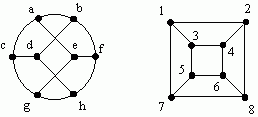
\includegraphics[width=2.2in]{figs/part2-isomorphic-graphs1.png}
\caption{Graphs to test isomorphism (1)}
\label{fig:part2-isomorphic-graphs1}
\end{minipage}%
\begin{minipage}{0.5\textwidth}
\centering
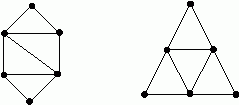
\includegraphics[width=2.2in]{figs/part2-isomorphic-graphs2.png}
\caption{Graphs to test isomorphism (2)}
\label{fig:part2-isomorphic-graphs2}
\end{minipage}
\end{figure}
\end{enumerate}




\vspace{10pt}
{\bf Trees}


\begin{enumerate}
%3.(a)
\item {\small \em  Given the count of vertices, edges, height or other parameter, estimate other parameters.}\\
There is a rooted tree $T$ with $100$ vertices; any inner node has no more than $2$ vertices.
\begin{enumerate}
\item Find the smallest possible number of leaves that can exist in $T$.
Find the largest number of leaves that can exist in $T$.
\item Find the smallest possible height of $T$.
\end{enumerate}

%3.(b)
\item {\small \em  Given an $n$-ary tree and some parameters, estimate other parameters.}\\
Let $T$ be a full $10$-ary tree with exactly $2021$ vertices.
\begin{enumerate}
\item Find the number of inner nodes in $T$.
\item Find the number of leaves in $T$.
\item Find the number of edges in $T$.
\item What can be the length of the longest path in $T$ (create $T$ so as
to make this path as long as possible).
\end{enumerate}



%3.(c)
\item {\small \em  Convert between representations: tree diagrams, lists of edges, or traversals.}\\
The post-order traversal of some rooted, ordered tree $T$ is as follows:
\[ v_{4}, v_{13}, v_{9}, v_{10}, v_{5}, v_{6}, v_{1}, v_{2}, v_{11}, v_{14},
v_{15}, v_{12}, v_{7}, v_{8}, v_{3}, v_{0}. \]
In this tree $v_0$, $v_1$ have tree children each; $v_3$, $v_5$, $v_7$, $v_{12}$ have
two children each; $v_{9}$ has one child.
\begin{enumerate}
\item Represent this tree as a diagram (root vertex at the very top; parents connected with
their children).
\item Represent this tree as adjacency lists (each edge in this tree is directed
from a parent to a child).
\end{enumerate}


%3.(d)
\item {\small \em  Given a prefix, infix or postfix notation, convert it into the syntax tree or other notation(s).}\\
Consider the following predicate-logic expression:
\[ \neg \bigg( \forall a \in H\ \exists b \in H\ \exists c \in H\ \Big( R(a)\ \vee\  \big(K(a,b) \wedge K(a,c) \wedge b \neq c \wedge R(b) \wedge R(c)\big) \Big) \bigg). \]
Boolean operations $\vee$ and $\wedge$ in this formula are {\em binary} (they
are nodes which need two children each),
boolean operation $\neg$ and all the quantifiers ($\forall a \in H$, $\exists b \in H$, etc.) are {\em unary} (they are nodes which need just one child),
but the predicates such as $R(a)$, $K(a,b)$ are leaves.

\begin{enumerate}
\item Draw the syntax tree for this predicate logic expression. Assume that disjunction and conjunction are both left-associative.
\item Visit all the vertices of this syntax tree in the pre-order sequence.
\end{enumerate}


%3.(e)
\item {\small \em  Given a directed or an undirected
graph, do a DFS and BFS traversal.}\\
Figures~\ref{fig:part2-directed-graph-dfs} and \ref{fig:part2-undirected-graph-dfs}
show directed and undirected graphs respectively.

Create their BFS and DFS trees (their roots are in vertices $A$ and $1$ respectively).
Visit all children in alphabetical order (or the order of increasing numbers).
If at some point you run out of vertices, pick the alphabetically smallest
vertex among the remaining ones and start the process.
You should create $4$ different trees (BFS for the directed graph;
BFS for the undirected graph; DFS for the directed graph; DFS for the undirected
graph).

{\em Note.} You do not need to show forward edges, back edges, cross edges in your
pictures; just the tree edges are enough.

\begin{figure}[!htb]
\centering
\begin{minipage}{.5\textwidth}
\centering
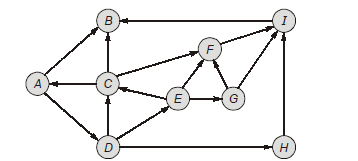
\includegraphics[width=2.6in]{figs/part2-directed-graph-dfs.png}
\caption{Directed graph for DFS/BFS}
\label{fig:part2-directed-graph-dfs}
\end{minipage}%
\begin{minipage}{0.5\textwidth}
\centering
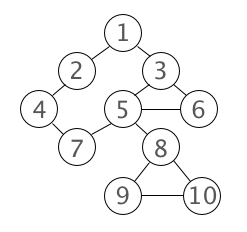
\includegraphics[width=1.25in]{figs/part2-undirected-graph-dfs.png}
\caption{Undirected graph for DFS/BFS}
\label{fig:part2-undirected-graph-dfs}
\end{minipage}
\end{figure}






\end{enumerate}



\end{document}
